\section{Analisi del prodotto esistente}

Al momento dell'arrivo in azienda \hl{era} già presente una versione alpha del software. \\
\hl{Le aziende che il prodotto si prefigge di supportare in questa fase, sono quelle con} i codici \gls{ATECO}\G\ in ambito edilizio. \hl{In particolare, al mio arrivo erano gestite} le informazioni relative a:
\begin{itemize}
	\item Sedi;
	\item Cantieri;
	\item Dipendenti;
	\item Organigramma aziendale;
	\item Abitabilità;
	\item Certificato di prevenzione degli incendi;
	\item \gls{DVR}\G\ e documentazione collaterale ad esso.
\end{itemize}
Il software espone\hl{va} una collezione di oltre 400 domande. Sulla base delle risposte a queste domande ed alle informazioni relative alle entità sopra indicate, \hl{venivano} verificati alcuni vincoli mediante regole del sistema esperto.

\subsection{Architettura del software}
\subsubsection{Architettura ad alto livello}
Il software è gestito mediante tecnologia \gls{SaaS}\G, un modello di distribuzione del software applicativo dove il fornitore del software si occupa della sua implementazione e manutenzione. Il servizio viene erogato al cliente mediante una applicazione web fruibile via internet. \\ 
L'applicazione web risiede fisicamente su una macchina virtuale della piattaforma cloud \gls{AWS}\G, al fine di evitare oneri e spese di gestione di una infrastruttura informatica dedicata e garantire la scalabilità del servizio.\\

Come è possibile osservare da \autoref{fig:Architettura}, ogni istanza di macchina virtuale contiene un clone dell'intera architettura. È stata scelta questa soluzione perché è prevista la possibilità di vendere il pacchetto a più utenti che possono fungere da distributori.\\
Ogni istanza è composta da quattro componenti principali:
\begin{itemize}
	\item \textit{Rule Engine;}
	\item \textit{Database;}
	\item \textit{Web Application;}
	\item \textit{Storage.}
\end{itemize}
La componente \textit{Storage}, in particolare, è stata dedicata al salvataggio di documenti in formato PDF esportabili in ogni momento da ogni azienda. Questa funzionalità non è ancora stata implementata. \\
Il routing delle richieste viene effettuato con un \gls{reverse proxy}\G, nello specifico \textit{NGINX}. \\
In particolare Ruby on Rails permette nativamente di creare e versionare i database a seconda dell'ambiente nel quale si opera (\textit{development, test, staging e production}). Questa caratteristica è tornata molto utile per lo sviluppo, dal momento che è stato possibile fare test accurati senza intaccare i dati in produzione. Inoltre ciò rende possibile evitare di utilizzare la console in sandbox di Rails, la quale presenta criticità nella consistenza dei dati visibili da shell ripetto a quelli visibili da \gls{browser}\G. \\
La persistenza dei dati è stata gestita mediante il modulo \texttt{ActiveRecord} di Ruby on Rails (descritto nella sezione \ref{sec:ActiveRecord}) il quale salva le informazioni su un database \textit{ PostgreSQL}.
\begin{figure}[H]
	\begin{center}
		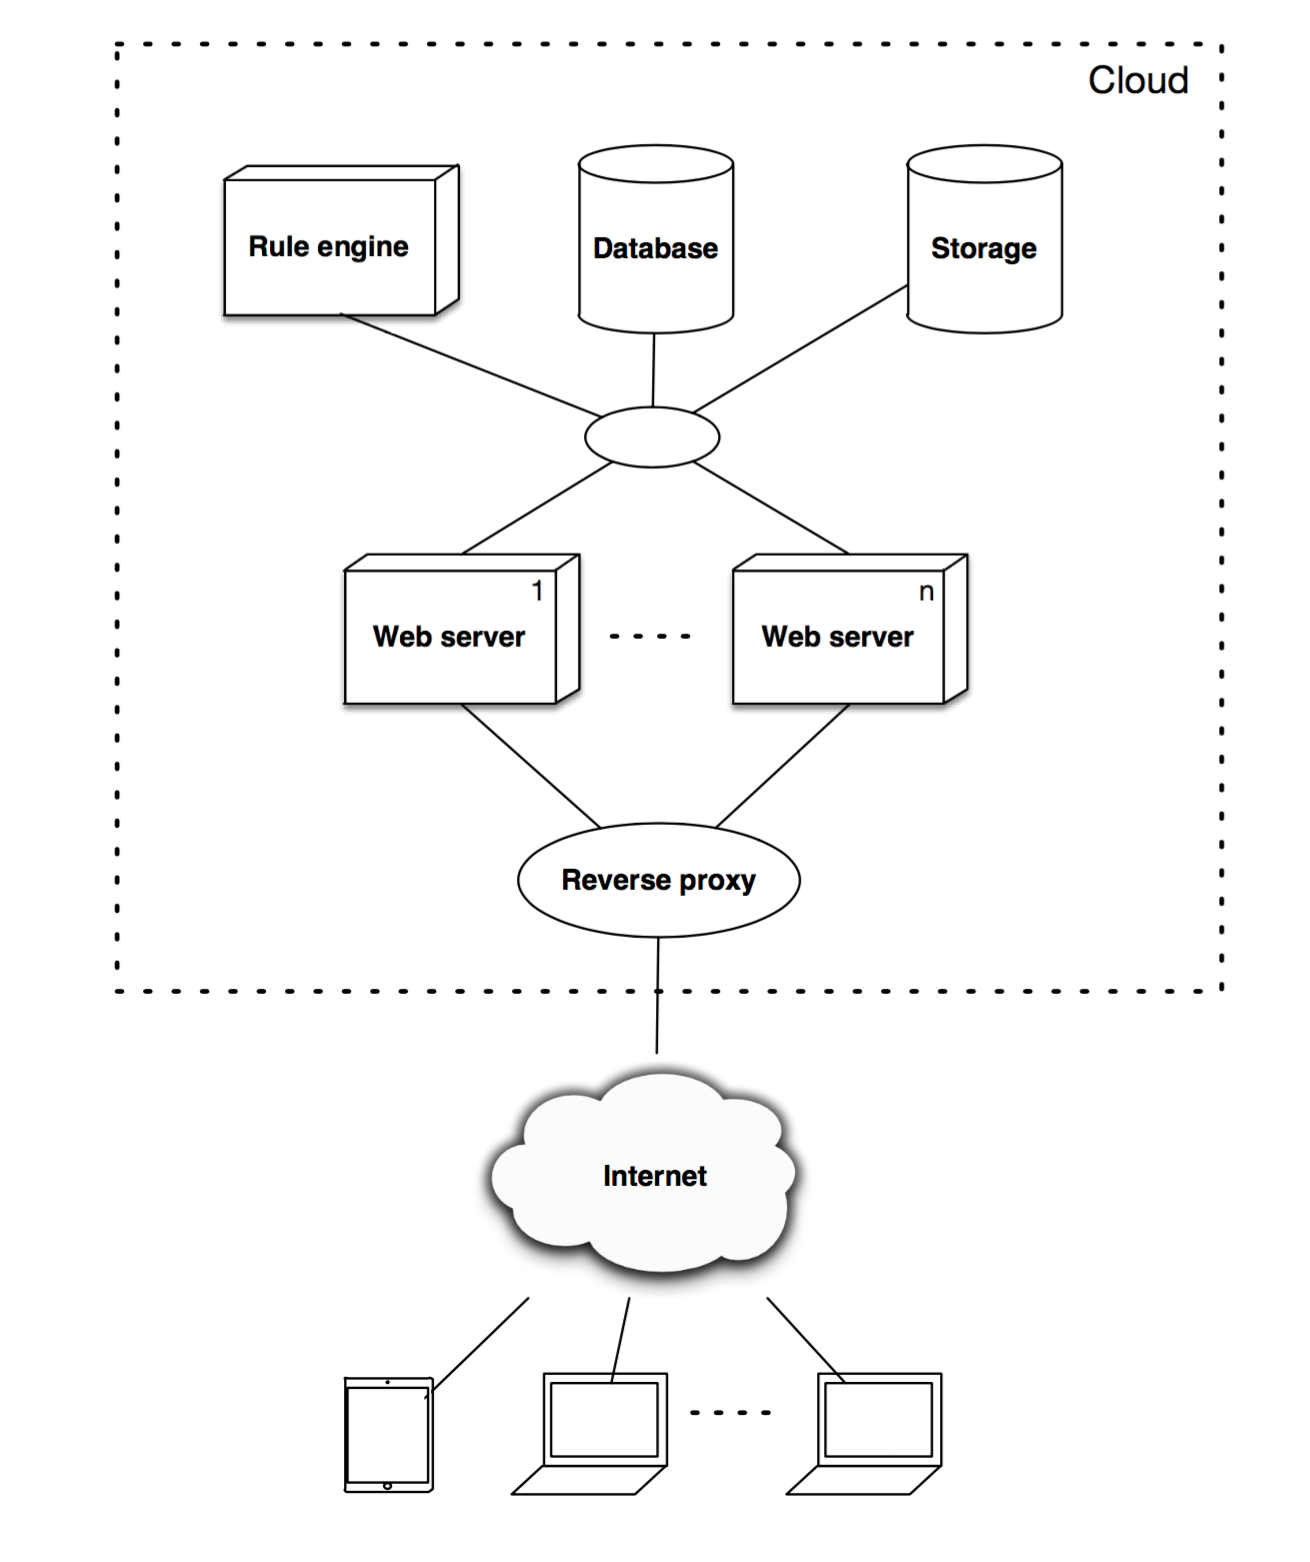
\includegraphics[width=16cm]{Pics/architettura.png}
		\caption{Architettura del sistema}
		\label{fig:Architettura}
	\end{center}
\end{figure}

\subsubsection{Architettura a basso livello}
L'applicazione web è organizzata secondo il pattern \gls{MVC}\G. Per il raggiungimento delle viste e l'accesso alle informazioni necessarie al corretto funzionamento dell'applicazione è stata implementata una interfaccia \gls{REST}\G. \\
Il sistema ha come entità principale il modello \texttt{Company} al quale sono riferite, direttamente o indirettamente, tutte le risorse.\\ 
Sono poi presenti numerosi modelli relativi alle entità che partecipano alla procedura di \gls{asseverazione}\G.
I modelli più significativi sono:
\begin{itemize} 
	\item \texttt{Alert} per rappresentare gli allarmi;
	\item \texttt{Answer} per rappresentare le risposte alle domande;
	\item \texttt{Company} per rappresentare una azienda;
	\item \texttt{ConstructionSite} per rappresentare un cantiere;
	\item \texttt{Dpi} per rappresentare un dispositivo di protezione individuale;
	\item \texttt{Duty} per rappresentare una mansione;
	\item \texttt{FireExtinguisher}  per rappresentare un estintore;
	\item \texttt{FirstAidBox} per rappresentare una cassetta di primo soccorso;
	\item \texttt{Individual} per rappresentare una persona;
	\item \texttt{Location} per rappresentare un edificio aziendale, ovvero una sede operativa, una sede amministrativa, una sede legale oppure un magazzino;
	\item \texttt{Machine, LiftingEquipment, ElectricTool}  per rappresentare un mezzo oppure uno strumento presente nel parco macchine;
	\item \texttt{MedicalVisit} per rappresentare una visita medica;
	\item \texttt{Procedure} per rappresentare una procedura aziendale, sia essa di prassi o di sistema;
	\item \texttt{Question} per rappresentare una domanda;
	\item \texttt{Training} per rappresentare un corso.
\end{itemize}	
Per ciascun modello, sono stati realizzati opportuni \textit{controller} e \textit{viste}. \\
Sono stati implementati, inoltre numerosi \gls{concern}\G\ per modularizzare le funzionalità indipendenti dalla singola classe ed allo stesso tempo riutilizzabili da altre classi. Ad esempio, ogni modello che, se istanziato, provoca un aumento del numero delle domande in attesa di risposta, include un apposito \gls{concern}\G\ per l'aggiornamento di un contatore dedicato a tale scopo. Per il calcolo del valore, il \gls{concern}\G\ ricava il nome della classe dell'oggetto corrente mediante \gls{reflection}\G\ ed incrementa automaticamente il valore del numero di domande correlate al tipo individuato.\\

\paragraph*{Relazioni tra domande, risposte ed allarmi}\mbox{} \\
Le risposte sono direttamente collegate alle domande ed ad una entità. Quando un utente risponde ad una domanda, viene aggiornato il recod relativo a quella risposta. A seguito di un inserimento o aggiornamento di una risposta, interviene Drools che valuta se le informazioni inserite rispettano tutti i vincoli previsti, altrimenti viene sollevato un allarme. \\ Per questioni di efficienza, gli allarmi relativi al vincolo di presenza  di una risposta, vengono gestiti direttamente dalle funzionalità di validazione di Rails.\\
Come per le answer, anche gli allarmi sono sempre collegati ad una risorsa, che di default è l'azienda corrente, ma può assumere come valore una qualsiasi istanza di un modello, purché non sia nulla.
Particolarmente degna di nota è l'associazione di una risposta o di un \textit{allarme} alla relativa risorsa. Per fare ciò si è utilizzato l'approccio standard di Rails per il supporto alle associazioni polimorfe. \\  Come si può vedere da  \autoref{fig:DiagrammaClassiAssociazioniPolimorfe}, indicando il tipo e l'id della risorsa interessata, l'accesso avviene tramite valutazione della classe e ricerca del relativo \textit{id}. \\
Si può pensare, ad esempio, all'allarme scatenato alla scadenza di un estintore. \\
La Risposta (\textit{Answer}) avrà i due campi \texttt{answerable\_type} ed \texttt{answerable\_id} impostati rispettivamente a \textit{"FireExtinguisher"} ed al suo \textit{id}.  L'allarme avrà un riferimento alla domanda per la quale è stata data una risposta. In questo modo è possibile conoscere il punto esatto dove dirottare l'utente al click sull'allarme per raggiungere il punto di non conformità. Questo aspetto è stato considerato di fondamentale importanza poiché la mole delle informazioni nel software è molto grande, è quindi necessario fornire il maggior numero di strumenti possibili all'utente per facilitarne la navigazione e l'orientamento nel sistema.
\begin{figure}[H]
	\begin{center}
		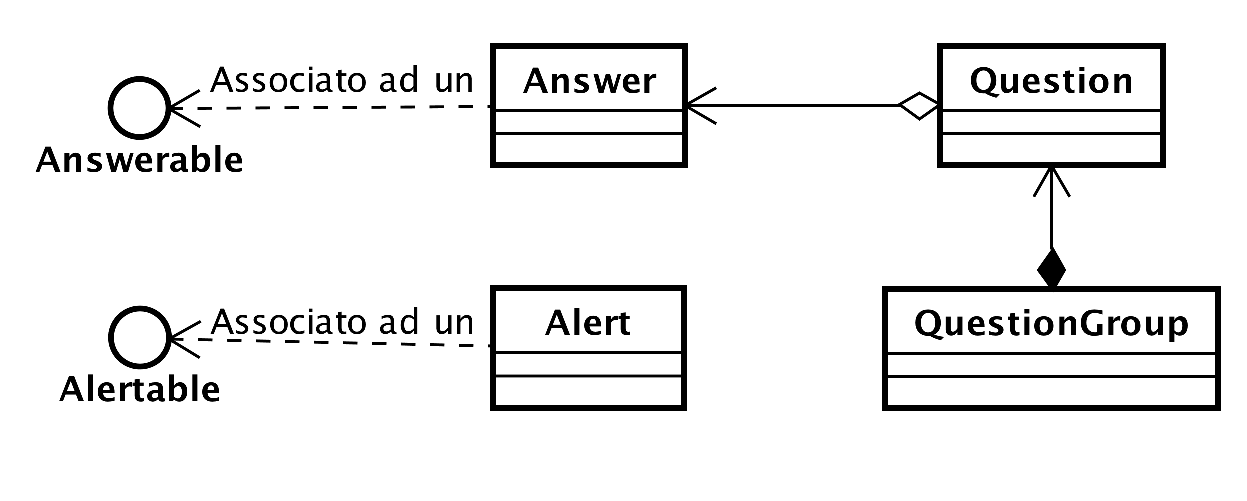
\includegraphics[width=14cm]{Pics/diagramma_classi_associazioni_polimorfe.png}
		\caption{Diagramma delle classi delle associazioni polimorfe di Risposte ed Allarmi.}
		\label{fig:DiagrammaClassiAssociazioniPolimorfe}
	\end{center}
\end{figure}

\subsubsection{Integrazione tra Ruby on Rails e Drools}\mbox{} \\

Il codice è stato scritto per la maggior parte utilizzando Ruby on Rails ma il rule engine (Drools) è un \gls{framework}\G\ scritto in Java. I due linguaggi non sono nativamente compatibili. \\
Per ovviare a questo problema, è stato utilizzato JRuby, un interprete del linguaggio Ruby scritto in Java, quindi in esecuzione su una \gls{JVM}\G\. \\
Per il corretto funzionamento di Drools, è necessario inserire le informazioni nella \textit{Working Memory} come \textit{"fatti"} che sono richiesti come oggetti di tipo \gls{JavaBean}\G\ o \gls{POJO}\G.\\
Per far cooperare i due ambienti, è stato implementato un apposito \gls{concern}\G\ chiamato \texttt{"act\_as\_fact"}. Questo modulo viene incluso nelle classi delle quali è necessario tenere traccia nella \textit{Working Memory} e vengono generati, mediante \gls{reflection} utilizzando i template di Rails (\gls{ERB}\G), le classi Java corrispondenti.




%\paragraph*{Criticità incontrate}\mbox{} \\
%\hl{SPOSTARE NELLA SEZIONE IN CUI SCRIVO QUELLO CHE HO FATTO IO}
%\hl{INSERIRE IL REMOTE TRUE NELLE VISTE}



\newpage
\subsubsection{Flusso dei dati ed interazione}

 Un aspetto che merita di essere esaminato è il flusso con il quale vengono generate e valutate domande e risposte .
\begin{figure}[H]
	\begin{center}
		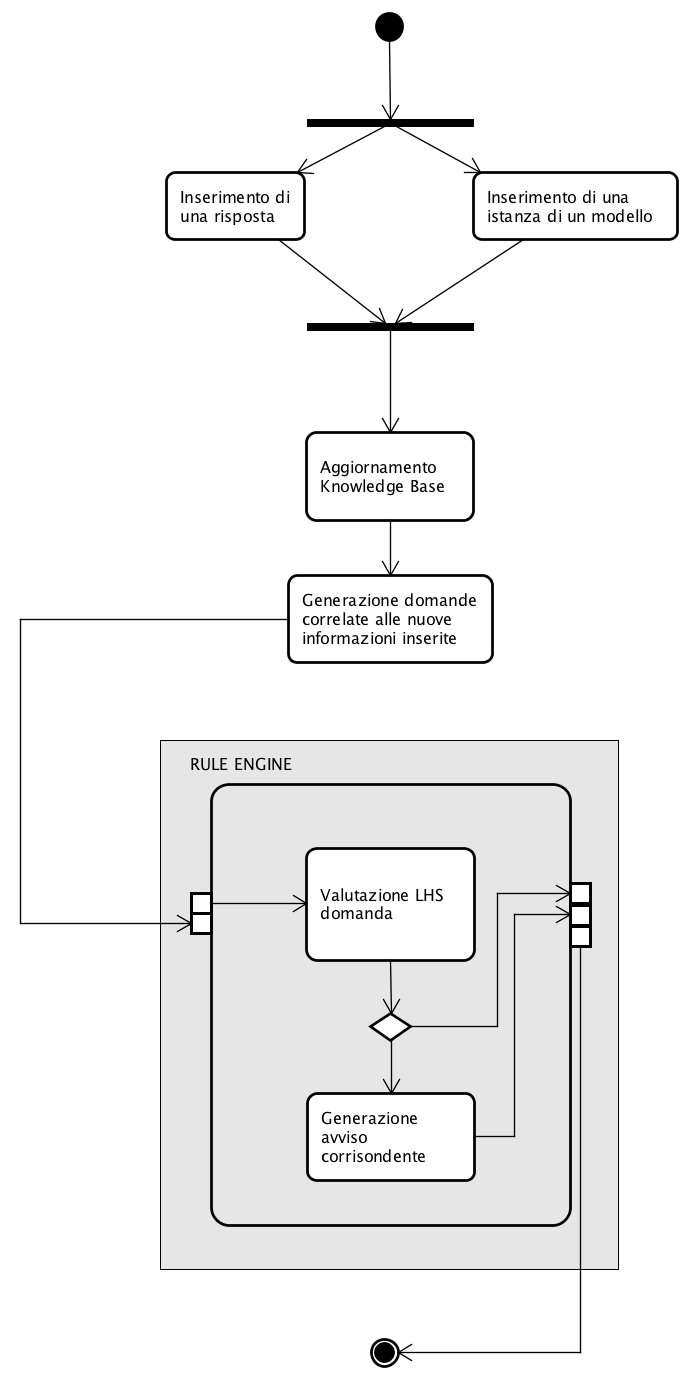
\includegraphics[width=8cm]{Pics/diagramma_attivita_risposte.png}
		\caption{Diagramma di attività del flusso di una risposta o l'inserimento di un oggetto a modello}
		\label{fig:DiagrammaAttivitaRisposte}
	\end{center}
\end{figure}

Come è possibile osservare dalla \autoref{fig:DiagrammaAttivitaRisposte}, nel momento in cui un utente inserisce o modifica un'istanza di un modello oppure risponde ad una domanda, viene aggiornata la \textit{Working Memory}. \\
Nel caso un cui venga generata o aggiornata un'istanza di modello, può essere necessario l'inserimento di alcune domande ad essa direttamente correlate.\\
Un esempio è rappresentato dall'aggiunta di un estintore ad un cantiere. Ad ogni estintore in ogni cantiere deve essere associata una posizione specifica che deve essere riportata nel layout di cantiere per permetterne il facile reperimento in caso di incendio. La posizione nel layout di un estintore è rappresentata dal software come una risposta ad una domanda in un apposito questionario generato ad ogni associazione di un estintore ad un cantiere. Se tale informazione non è specificata viene sollevato un allarme.\\
Sia per l'inserimento o aggiornamento di una risposta, sia per la generazione o modifica di una istanza di modello, il passo successivo è rappresentato dalla valutazione delle informazioni inserite sulla base della \textit{Knowledge Base}. \\
È in questo momento che agisce il rule engine Drools che per ogni regola presente nella \textit{Knowledge Base} valuta la \gls{LHS}\G\ sulle nuove informazioni inserite e, se soddisfatta, solleva gli allarmi corrispondenti. 
Un esempio di regola è il seguente:


\begin{verbatim}
rule "Individuo ricopre una mansione per la quale non è formato"
	when
		$t: Training()
		$d: Duty(trainings contains $t)
		$i: Individual(duties contains $d, trainings not contains $t)
	then
		System.out.println($i.getFirstName() + ' ' + $i.getLastName() + "ha la mansione" +
		$d.getName() + " ma non la formazione " + $t.getName() );
end
\end{verbatim}
\begin{itemize}
	\item \$t contiene tutte le formazioni;
	\item \$d contiene  tutte le mansioni che necessitano della formazione \$t;
	\item \$i contiene tutti gli individui che svolgono la mansione \$d ma non sono in possesso della formazione \$t.
\end{itemize}
Le corrispondenze di questa regola sono tutti gli individui individui che svolgono una qualunque mansione per la quale non sono correttamente formati.\\
Al verificarsi di queste condizioni, viene generato un allarme il cui contenuto è specificato dalla stampa disposta dalla \gls{RHS}\G.


\cleardoublepage

\section{Definizione dei casi d'uso}
\hl{Nuovo capitolo}
	\subsection{Legenda}
	\begin{itemize}
		\item \texttt{UC:} Sigla utilizzata come abbreviazione per indicare un caso d'uso (\textit{Use Case});
		\item \texttt{Utente amministratore:} Utente che ha effettuato con successo il login nel sistema con privilegi da amministratore;
		\item \texttt{Utente autenticato:} Utente che ha effettuato con successo il login nel sistema.
	\end{itemize}
	
	\subsection{Tracciamento Casi d'uso - Requisiti}
		\hl{TODO: Tabella tracciamento Requisiti  - Casi d'uso}
	\subsection{Caso d'uso UCP - Scenario Principale }
	\hl{nuova sezione} \\
	\begin{figure}[H]
		\begin{center}
			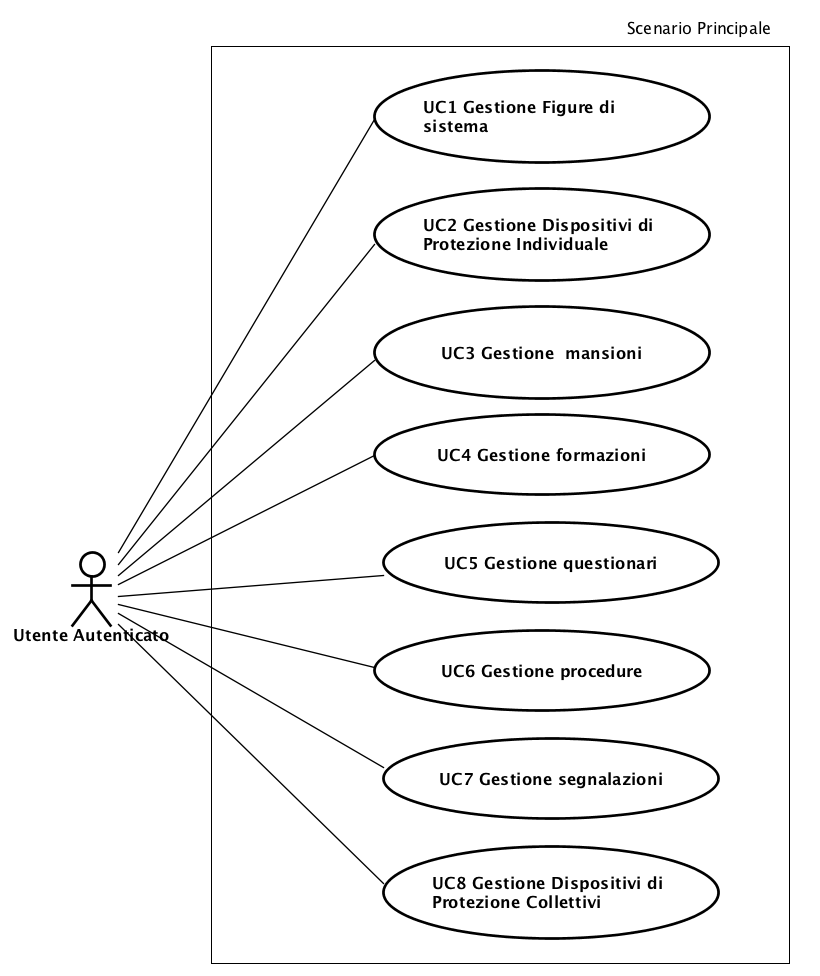
\includegraphics[width=11cm]{Pics/Diagramma_generale_dei_casi_d_uso.png}
			\caption{
				Diagramma dei casi d'uso generale.}
			\label{fig:DiagrammaGeneraleCasiDuso}
		\end{center}
	\end{figure}	
	
	\begin{itemize}
		\item \textbf{Scopo:} Il diagramma generale dei casi d'uso UCP (\autoref{fig:DiagrammaGeneraleCasiDuso}), ha lo scopo di rappresentare ad alto livello i casi d'uso necessari al soddisfacimento di tutti i requisiti. \\
		In particolare un utente che abbia effettuato con successo il login nel sistema, deve poter gestire: figure di sistema; dispositivi di protezione individuali, mansioni, formazioni, questionari, procedure; segnalazioni e dispositivi di protezione collettivi.
		A seguire la spiegazione e l'esplosione in sotto casi d'uso per ognuno dei casi d'uso sopra elencati.
		\item \textbf{Attori Coinvolti:} Utente Autenticato;
		\item \textbf{Flusso principale degli eventi:} 
			\begin{itemize}
				\item \textit{L'utente autenticato gestisce le Figure di sistema (\hyperref[section:UC1]{UC1});}
				\item \textit{L'utente autenticato gestisce i Dispositivi di Protezione individuale (\hyperref[section:UC2]{UC2});}
				\item \textit{L'utente autenticato gestisce le mansioni (\hyperref[section:UC3]{UC3});}
				\item \textit{L'utente autenticato gestisce le formazioni (\hyperref[section:UC4]{UC4});}
				\item \textit{L'utente autenticato gestisce i questionari (\hyperref[section:UC5]{UC5});}
				\item \textit{L'utente autenticato gestisce le procedure (\hyperref[section:UC6]{UC6});}
				\item \textit{L'utente autenticato gestisce le segnalazioni (\hyperref[section:UC7]{UC7})}
				\item \textit{L'utente autenticato gestisce i dispositivi di protezione collettivi (\hyperref[section:UC8]{UC8}).}
			\end{itemize}
	\end{itemize}
	

	\subsection{UC1 Gestione delle Figure di sistema}
	\label{section:UC1}
	\hl{Nuova sezione}
	\begin{figure}[H]
		\begin{center}
			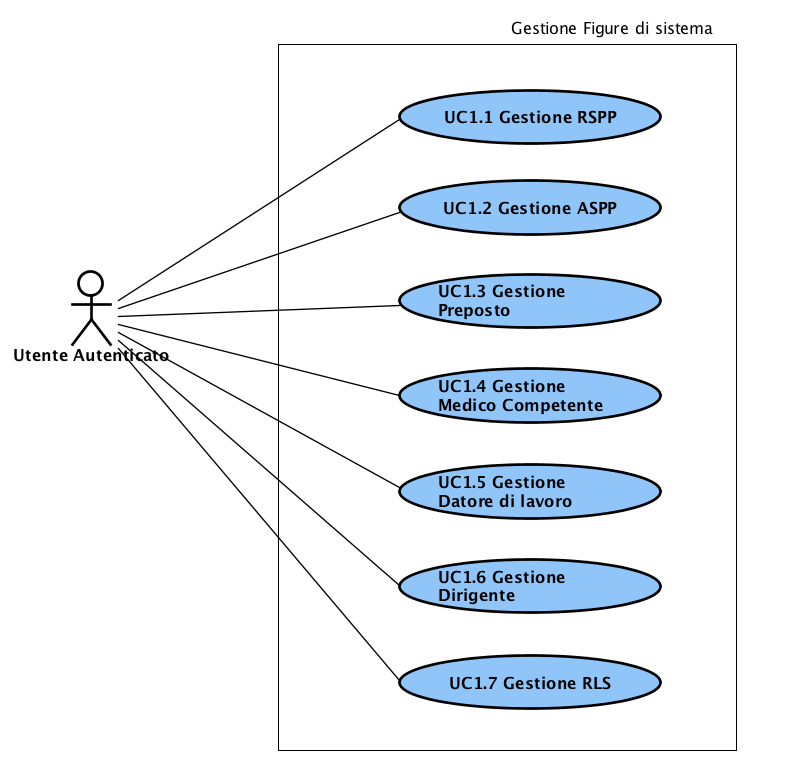
\includegraphics[width=10cm]{Pics/UC1GestioneFigureDiSistema.png}
			\caption{
				Diagramma dei casi d'uso UC1 - Figure di sistema.}
			\label{fig:UC1GestioneFigureDiSistema}
		\end{center}
	\end{figure}
	\begin{itemize}
		\item \textbf{Scopo:} Il diagramma generale dei casi d'uso UC1 (\autoref{fig:UC1GestioneFigureDiSistema}), ha lo scopo di rappresentare ad alto livello i casi d'uso necessari al soddisfacimento di tutti i requisiti rigruardanti le figure di sistema;
		\item \textbf{Attori Coinvolti:} Utente Autenticato;
		\item \textbf{Flusso principale degli eventi:} 
		\begin{itemize}
			\item \textit{L'utente autenticato gestisce gli RSPP (\hyperref[section:UC1_1]{UC1.1});}
			\item \textit{L'utente autenticato gestisce gli ASPP (UC1.2);}
			\item \textit{L'utente autenticato gestisce i preposti (UC1.3);}
			\item \textit{L'utente autenticato gestisce il medico competente (UC1.4);}
			\item \textit{L'utente autenticato gestisce il datore di lavoro (UC1.5);}
			\item \textit{L'utente autenticato gestisce i dirigenti (UC1.6);}
			\item \textit{L'utente autenticato gestisce gli RLS (UC1.7).}
		\end{itemize}
	\end{itemize}
		
	\subsection{UC1.1 Gestione degli RSPP}
	\label{section:UC1_1}
	\hl{Nuova sezione}
	Tutte le figure di sistema presentano requisiti analoghi. Per evitare di affaticare la lettura con sezioni ridondanti è stato scelto di riportare soltanto il diagramma dei casi d'uso riguardante gli RSPP. Si intende che per tutte le altre figure di sistema il diagramma sia analogo. 
		\begin{figure}[H]
			\begin{center}
				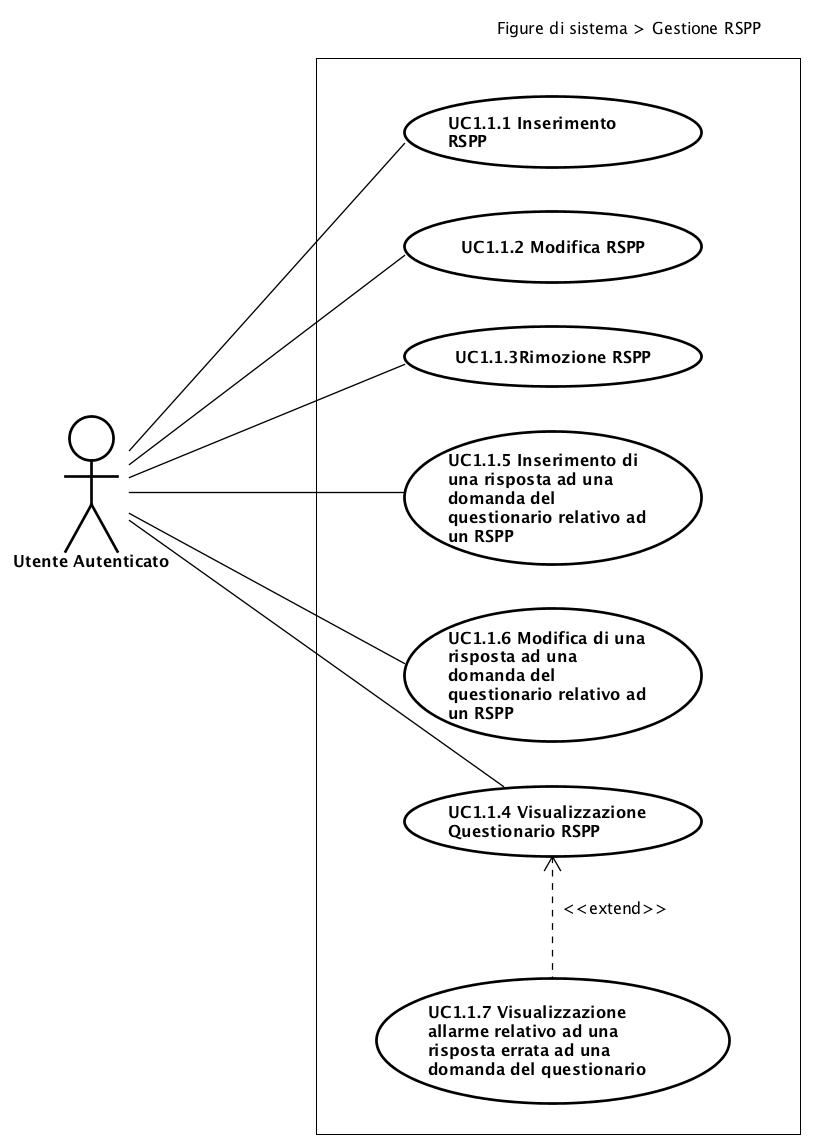
\includegraphics[width=12cm]{Pics/UC1_1_FigureDiSistema_RSPP.png}
				\caption{Diagramma dei casi d'uso relativo all'inserimento degli RSPP}
				\label{fig:UC1_1RSPP}
			\end{center}
		\end{figure}
		\begin{itemize}
			\item \textbf{Scopo:} Il diagramma relativo alla gestione degli RSPP (\autoref{fig:DiagrammaGeneraleCasiDuso}), ha lo scopo di rappresentare i casi d'uso necessari al soddisfacimento di tutti i requisiti riguardanti la gestione degli RSPP. \\
			In particolare un utente che abbia effettuato con successo il login nel sistema, deve poter inserire, rimuovere, modificare  RSPP. Deve essere messo in condizione inoltre di Visualizzare un questionario relativo ad uno specifico RSPP, rispondendo alle domande riportate su di esso. In caso di errore, deve essere sollevato un allarme che comunica la domanda esatta ed un messaggio esplicativo.
			\item \textbf{Attori Coinvolti:} Utente Autenticato;
			\item \textbf{Flusso principale degli eventi:} 
			\begin{itemize}
				\item \textit{L'utente autenticato inserisce un RSPP (UC1.1.1);}
				\item \textit{L'utente autenticato modifica un RSPP(UC1.1.2);}
				\item \textit{L'utente autenticato rimuove un RSPP (UC1.1.3);}
				\item \textit{L'utente autenticato visualizza il questionario associato ad un RSPP (UC1.1.4);}
				\item \textit{L'utente autenticato inserisce una risposta ad una domanda del questionario (UC1.1.5);}
				\item \textit{L'utente autenticato modifica di una risposta ad una domanda del questionario relativo ad un RSPP (UC1.1.6);}
				\item \textit{ L'utente autenticato visualizza un allarme relativo ad una risposta errata ad una domanda del questionario (UC1.1.7).}
			\end{itemize}
		\end{itemize}
	\newpage	
	\subsection{UC2 Gestione dei Dispositivi di Protezione Individuale (DPI)}
		\label{section:UC2}
		\hl{Nuova sezione}
		La gestione dei  \gls{DPI}\G\ va suddivisa in due scenari distinti. Il primo scenario è relativo alla gestione delle tipologie di \gls{DPI}\G\ disponibili da parte degli utenti amministratori. Il secondo scenario riguarda la gestione dei \gls{DPI}\G\ che compongono la dotazione personale di un dipendente. \\
		Seguono i diagrammi dei casi d'uso dei \gls{DPI}\G\ relativi agli scenari sopra indicati.

		\subsubsection{UC2.1 Gestione delle tipologie di DPI dal pannello di amministrazione }
			\label{section:UC2_1}
			\hl{Nuova sezione}
			\begin{figure}[H]
				\begin{center}
					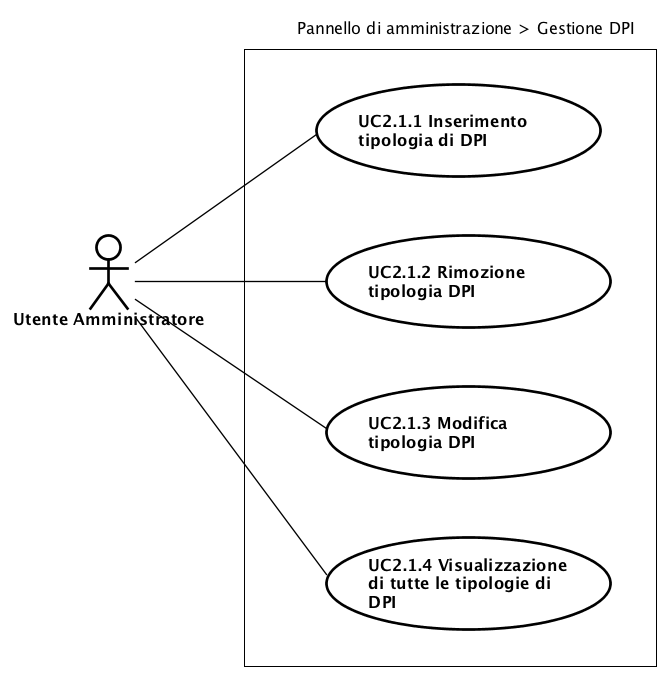
\includegraphics[width=12cm]{Pics/UC2_1GestioneDispositiviDiProtezioneIndividualeDaPannelloDiAmministrazione.png}
					\caption{
						Diagramma dei casi d'uso UC2.1 - Gestione tipologie di DPI dal pannello di amministrazione.}
					\label{fig:UC2_1GestioneDPIAmministrazione}
				\end{center}
			\end{figure}
			\begin{itemize}
				\item \textbf{Scopo:} Il diagramma presentato nella \autoref{fig:UC2_1GestioneDPIAmministrazione}, ha lo scopo di rappresentare i casi d'uso necessari al soddisfacimento di tutti i requisiti riguardanti la gestione delle tipologie dei \gls{DPI}\G.
				 \\ Un utente amministratore deve poter gestire in modo autonomo le tipologie di \gls{DPI}\G\ che ritiene più opportune e metterle a disposizione degli utilizzatori del sistema.
				\item \textbf{Attori Coinvolti:} Utente Amministratore;
				\item \textbf{Flusso principale degli eventi:} 
				\begin{itemize}
					\item \textit{L'utente amministratore inserisce una tipologia di \gls{DPI}\G\ (UC2.1.1);}
					\item \textit{L'utente amministratore rimuove una tipologia di \gls{DPI}\G\ (UC2.1.2);}
					\item \textit{L'utente amministratore modifica una tipologia di \gls{DPI}\G\ (UC2.1.3);}
					\item \textit{L'utente amministratore visualizza tutte le tipologie di \gls{DPI}\G\ (UC2.1.3).}
				\end{itemize}
			\end{itemize}
		\subsubsection{UC2.2 Gestione dei DPI assegnati ai dipendenti}
		\hl{Nuova sezione}
			\label{section:UC2_2}
			\begin{figure}[H]
				\begin{center}
					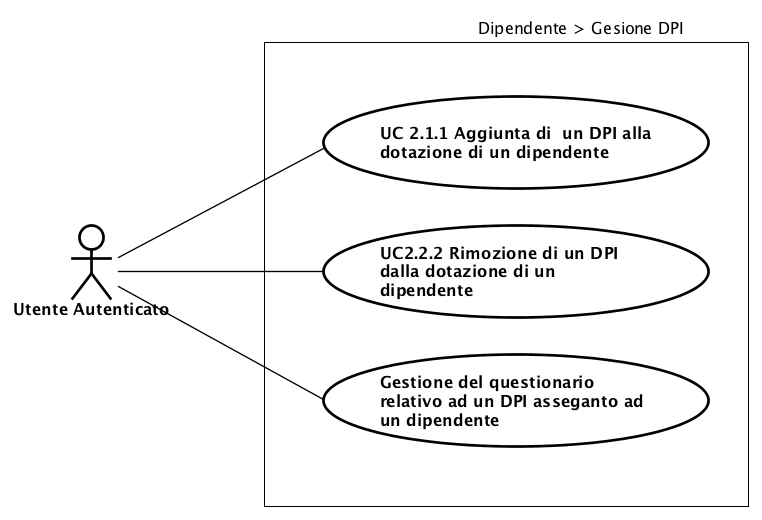
\includegraphics[width=12cm]{Pics/UC2_2DPIDipendenti.png}
					\caption{
						Diagramma dei casi d'uso UC2.2 - Gestione dei DPI relativi ad un dipendente.}
					\label{fig:UC2_2GestioneDPIDipendenti}
				\end{center}
			\end{figure}
			\begin{itemize}
				\item \textbf{Scopo:} Il diagramma presentato nella \autoref{fig:UC2_2GestioneDPIDipendenti}, ha lo scopo di rappresentare i casi d'uso necessari al soddisfacimento di tutti i requisiti riguardanti la gestione dei \gls{DPI}\G\ dati in dotazione ai dipendenti. \\ Un utente autenticato deve poter assegnare o rimuovere \gls{DPI}\G\ ad ogni dipendente. Deve essere possibile assegnare \gls{DPI}\G\ con molteplicità variabile, scegliendo la tipologia da una lista predefinita (Sezione: \ref{section:UC2_1}).\\
				Per ogni \gls{DPI}\G\ deve essere possibile rispondere ad un questionario;
				\item \textbf{Attori Coinvolti:} Utente Autenticato;
				\item \textbf{Flusso principale degli eventi:} 
				\begin{itemize}
					\item \textit{L'utente autenticato aggiunge un \gls{DPI}\G\ alla dotazione di un dipendente (UC2.2.1);}
					\item \textit{L'utente autenticato rimuove un \gls{DPI}\G\ dalla dotazione di un dipendente  (UC2.2.2);}
					\item \textit{L'utente autenticato gestisce il questionario relativo ad un \gls{DPI}\G\ assegnato ad un dipendente (UC2.2.3);}
					\item \textit{L'utente autenticato visualizza tutti i \gls{DPI}\G\ assegnati ad un dipendente (UC2.2.4).}
				\end{itemize}
			\end{itemize}
	\newpage		
	\subsection{UC3 Gestione  delle mansioni}
		\label{section:UC3}
		\hl{Nuova sezione}\\
		\hl{Va bene un approccio di questo tipo oppure è preferibile riportare la descrizione anche in contesti come questo?}\\
		Le mansioni rappresentano le attività che un individuo interno all'azienda è abilitato a svolgere.\\
		L'associazione agli individui e la gestione delle mansioni disponibili è stato eseguito allo stesso modo dei \gls{DPI}\G. \\
		Per evitare di affaticare la lettura con sezioni ridondanti è stato scelto di riportare soltanto il diagramma dei casi d'uso riguardante i \gls{DPI}\G. Si intende che per le mansioni il diagramma e la spiegazione del caso d'uso sia analogo alla sezione \ref{section:UC2_2}.
	
	\newpage 
	\subsection{UC4 Gestione delle formazioni}
		\label{section:UC4}
		\hl{Nuova sezione}
		Con il termine formazione si intende una certificazione relativa ad un corso abilitante ad una o più mansioni.\\
		La gestione delle formazioni è del tutto simile a quella dei \gls{DPI}\G, fatta eccezione per la gestione delle scadenze. È richiesto infatti che un utente amministratore possa assegnare un periodo di validità della formazione in mesi dal pannello di controllo. Un utente autenticato deve visualizzare un allarme nel momento in cui una formazione sia scaduta.
		
	\subsubsection{UC4.1 Gestione delle formazioni dal pannello di amministrazione }

		\hl{Nuova sezione}\\
		Tutte le considerazioni della sezione \ref{section:UC2_2} valgono anche per le formazioni. \\
		A differenza dei \gls{DPI}\G\ va inserita una informazione aggiuntiva obbligatoria: il periodo di validità della formazione. \\
		Il diagramma dei casi d'uso è del tutto analogo a quello della  \autoref{fig:UC2_1GestioneDPIAmministrazione}.
	
	\subsubsection{UC4.2 Gestione delle formazioni dei dipendenti e del datore di lavoro }
		\hl{nuova sezione}\\
		\begin{figure}[H]
			\begin{center}
				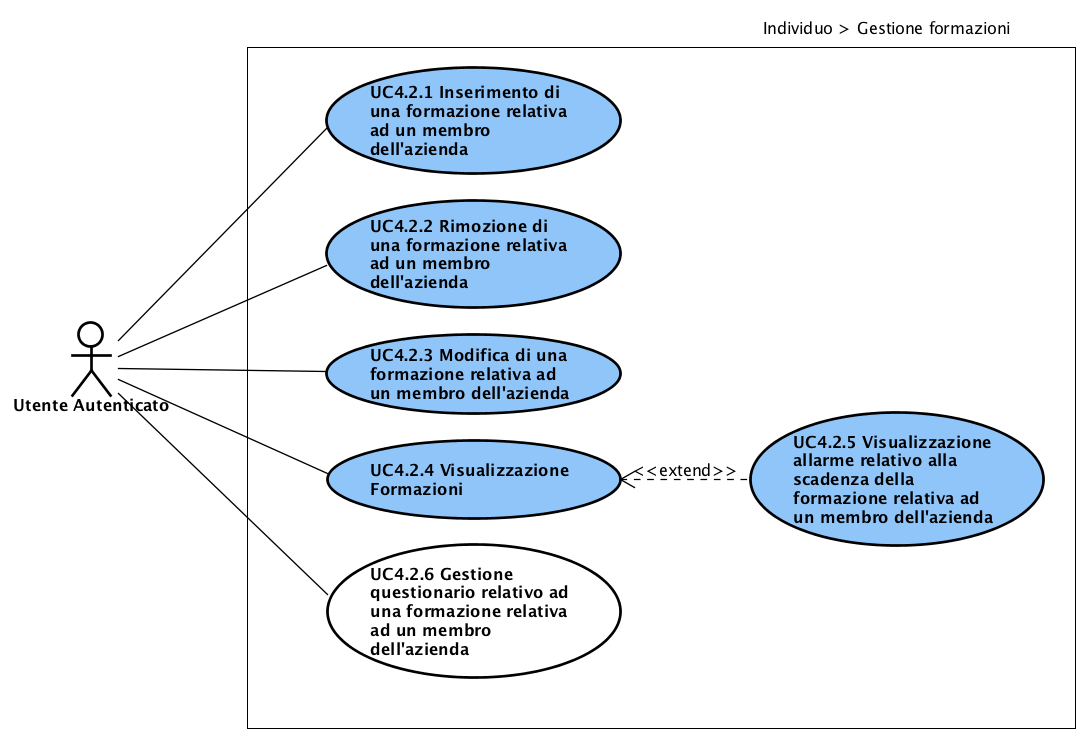
\includegraphics[width=16cm]{Pics/UC4_2GestioneFormazioni.png}
				\caption{Diagramma dei casi d'uso relativo alla gestione delle formazioni di un dipendente.}
				\label{fig:UC4_2_Formazioni}
			\end{center}
		\end{figure}
		
		\begin{itemize}
			\item \textbf{Scopo:} Il diagramma presentato nella \autoref{fig:UC4_2_Formazioni}, ha lo scopo di rappresentare i casi d'uso necessari al soddisfacimento di tutti i requisiti riguardanti la gestione delle formazioni relative ad un qualunque membro dell'azienda. \\ 
			Un utente autenticato deve poter assegnare o rimuovere formazioni ad ogni dipendente. 
			Ogni formazione relativa ad un dipendente deve essere dotata di un questionario. \\ 
			La scadenza della formazione deve essere segnalata trenta giorni prima della data ultima mediante un allarme.
			\item \textbf{Attori Coinvolti:} Utente Autenticato;
			\item \textbf{Flusso principale degli eventi:} 
			\begin{itemize}
				\item \textit{L'utente autenticato aggiunge una formazione ad un membro dell'azienda indicando descrizione e data (UC4.2.1);}
				\item \textit{L'utente autenticato rimuove una formazione ad un membro dell'azienda (UC4.2.2);}
				\item \textit{L'utente autenticato modifica una formazione ad un membro dell'azienda (UC4.2.3);}
				\item \textit{L'utente autenticato visualizza le formazioni relative ad un membro dell'azienda (UC4.2.4);}
				\item \textit{L'utente autenticato visualizza l'allarme relativo alla scadenza di una formazione in possesso di un membro dell'azienda (UC4.2.5);}
				\item \textit{L'utente autenticato gestisce il questionario relativo ad una formazione in possesso di un membro dell'azienda (UC4.2.6).}
			\end{itemize}
		\end{itemize}
		
	\newpage	
	\subsection{UC5 Gestione dei questionari}
		\label{section:UC5}	
			\begin{figure}[H]
				\begin{center}
					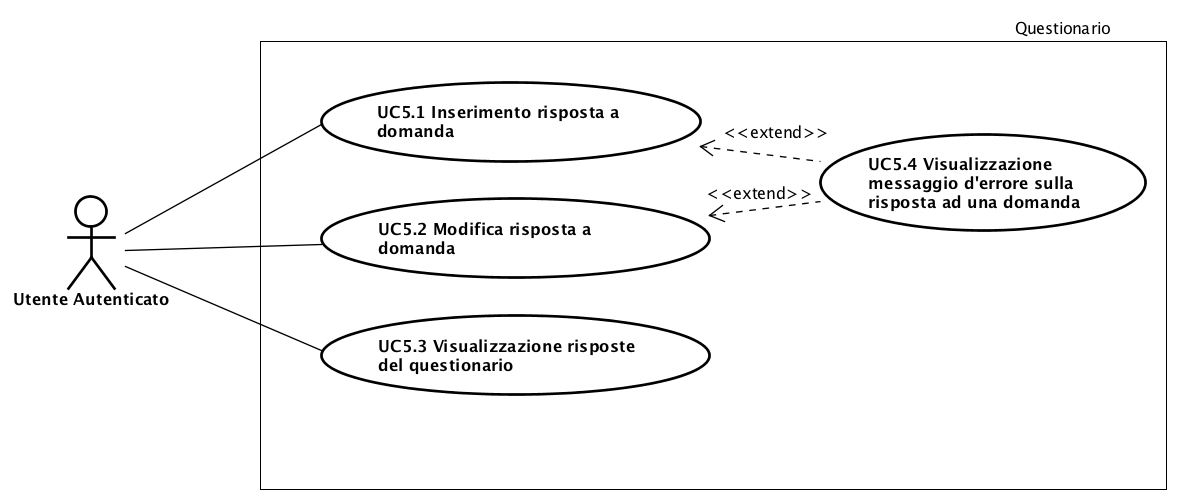
\includegraphics[width=15cm]{Pics/UC5QuestionarioUtenteAutenticato.png}
					\caption{Diagramma dei casi d'uso relativo alla gestione di un questionario.}
					\label{fig:UC5_Qestionari}
				\end{center}
			\end{figure}
			
			\begin{itemize}
				\item \textbf{Scopo:} Il diagramma presentato nella \autoref{fig:UC5_Qestionari}, ha lo scopo di rappresentare i casi d'uso necessari al soddisfacimento dei requisiti riguardanti la gestione di un questionario di pertinenza di un utente autenticato. \\ 
				Gli utenti amministratori devono poter gestire le domande poste nei questionari da un pannello d'amministrazione. Questo aspetto non è stato trattato in dettaglio poiché analogo a quanto descritto nella sezione \ref{section:UC2_1}.
				\item \textbf{Attori Coinvolti:} Utente Autenticato;
				\item \textbf{Flusso principale degli eventi:} 
				\begin{itemize}
					\item \textit{L'utente autenticato risponde per la prima volta ad una domanda (UC5.1);}
					\begin{itemize}
						\item \textit{Viene mostrato un messaggio d'errore se la risposta fornita non è corretta (UC5.4);}
					\end{itemize}
					\item \textit{L'utente autenticato modifica una risposta ad una domanda (UC5.2);}
					\begin{itemize}
						\item \textit{Viene mostrato un messaggio d'errore se la risposta fornita non è corretta (UC5.4);}
					\end{itemize}
					\item \textit{L'utente autenticato visualizza tutte le risposte al questionario (UC5.3). Se è la prima volta che lo apre, le risposte saranno tutte vuote.}
				\end{itemize}
			\end{itemize}
	
	\newpage		
	\subsection{UC6 Gestione delle procedure}
		\label{section:UC6}
		\hl{Nuova sezione}
		Le procedure rappresentano un aspetto di primaria importanza e si suddividono in due categorie: di prassi e di sistema. \\
		Le procedure si prassi derivano direttamente da un documento fornito dall'\gls{INAIL}\G. Queste procedure sono state individuate dall'analisi delle cause di infortunio maggiormente frequenti rilevate dall'\gls{INAIL}\G nel tempo allo scopo di migliorare la sicurezza dei lavoratori.
		Le procedure di sistema, invece, sono stese dall'azienda e fanno parte del \gls{DVR}\G. 
		\begin{figure}[H]
			\begin{center}
				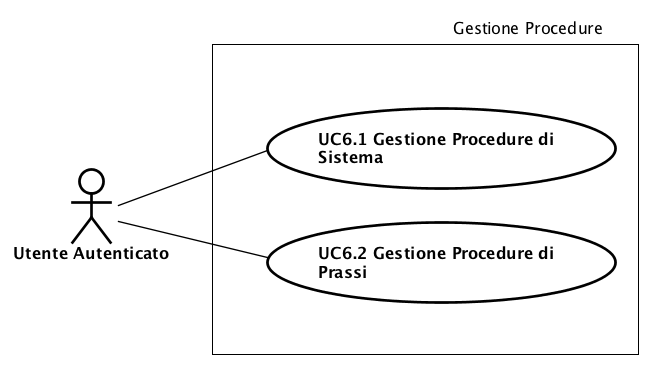
\includegraphics[width=12cm]{Pics/UC6GestioneProcedure.png}
				\caption{Diagramma dei casi d'uso relativo alla gestione delle procedure.}
				\label{fig:UC6_Procedure}
			\end{center}
		\end{figure}
		
			\begin{itemize}
				\item \textbf{Scopo:} Il diagramma presentato nella \autoref{fig:UC6_Procedure}, ha lo scopo di rappresentare i casi d'uso necessari alla gestione delle procedure all'interno dell'azienda. \\ 
				
				Un utente autenticato deve poter gestire procedure ad ogni dipendente. \\
				Ogni procedura, di sistema, deve essere dotata di Descrizione, Codifica e informazioni relative alle revisioni delle quali è stata oggetto nel tempo.\\
				Le procedure di prassi sono state gestite con un questionario (vedi sezione: \ref{section:UC5}) in quanto derivanti direttamente da una lista di domande proveniente dall'\gls{INAIL}\G;
				\item \textbf{Attori Coinvolti:} Utente Autenticato;
				\item \textbf{Flusso principale degli eventi:} 
				\begin{itemize}
					\item \textit{L'utente autenticato gestisce le procedure di sistema(UC6.1);}
					\begin{itemize}
						\item \textit{L'utente autenticato inserisce una nuova procedura di sistema(UC6.1.1);}
						\item \textit{L'utente autenticato modifica una procedura di sistema(UC6.1.2);}
						\item \textit{L'utente autenticato rimuove una procedura di sistema(UC6.1.3);}
						\item \textit{L'utente autenticato visualizza tutte le procedure di sistema(UC6.1.4).}
					\end{itemize}
					\item \textit{L'utente autenticato gestisce le procedure di prassi (UC6.2);}
					\begin{itemize}
						\item \textit{L'utente autenticato inserisce una nuova procedura di prassi (UC6.2.1);}
						\item \textit{L'utente autenticato modifica una procedura di prassi (UC6.2.2);}
						\item \textit{L'utente autenticato rimuove una procedura di prassi (UC6.2.3);}
						\item \textit{L'utente autenticato visualizza tutte le procedure di prassi (UC6.2.4).}
					\end{itemize}
				\end{itemize}
			\end{itemize}
			
	\newpage
	\subsection{UC7 Gestione delle segnalazioni}
		\label{section:UC7}	
		Le segnalazioni sono delle comunicazioni ufficiali indirizzate all'organo di vigilanza. Esse sono dotate di: descrizione, segnalante, data di comunicazione del segnalante all'alta direzione, data di comunicazione dall'alta direzione all'organo di vigilanza, data di risposta dell'organo di vigilanza al soggetto interessato.\\
		\begin{figure}[H]
			\begin{center}
				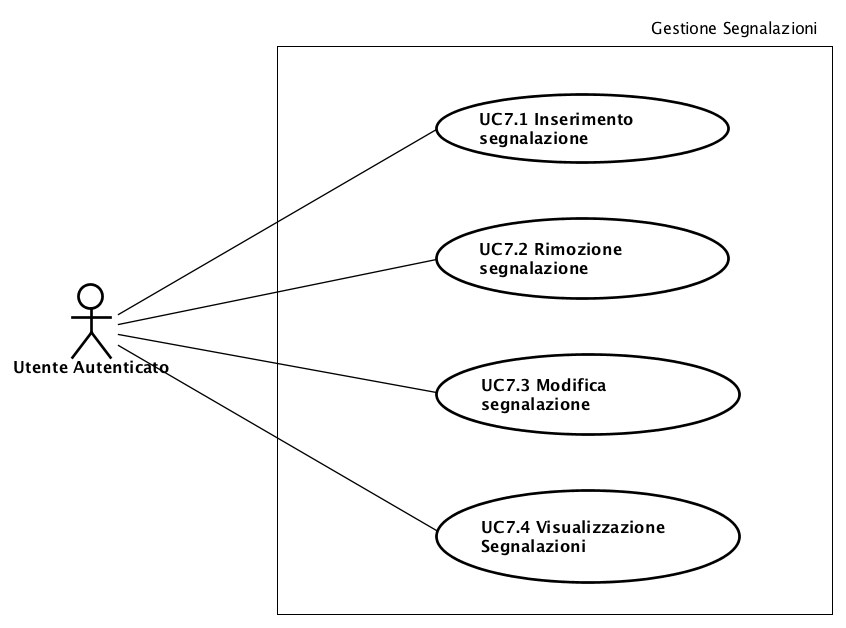
\includegraphics[width=12cm]{Pics/UC7Segnalazioni.png}
				\caption{Diagramma dei casi d'uso relativo alla gestione delle segnalazioni.}
				\label{fig:UC7_Segnalazioni}
			\end{center}
		\end{figure}
		
		\begin{itemize}
			\item \textbf{Scopo:} Il diagramma presentato nella \autoref{fig:UC7_Segnalazioni}, ha lo scopo di rappresentare i casi d'uso necessari al soddisfacimento di tutti i requisiti riguardanti la gestione delle segnalazioni all'interno dell'azienda. \\ 
			\item \textbf{Attori Coinvolti:} Utente Autenticato;
			\item \textbf{Flusso principale degli eventi:} 
			\begin{itemize}
				\item \textit{L'utente autenticato inserisce una segnalazione (UC7.1);}
				\item \textit{L'utente autenticato rimuove una segnalazione (UC7.2);}
				\item \textit{L'utente autenticato modifica una segnalazione (UC7.3);}
				\item \textit{L'utente autenticato visualizza tutte le segnalazioni (UC7.4);}
			\end{itemize}
		\end{itemize}
		
	\newpage	
	\subsection{UC8 Gestione dei Dispositivi di Protezione Collettivi}
		\label{section:UC8}
		\hl{Nuova sezione}
		\begin{figure}[H]
			\begin{center}
				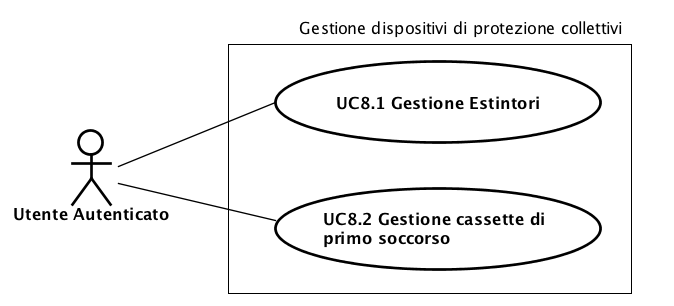
\includegraphics[width=12cm]{Pics/UC8GestioneDispositiviProtezioneCollettivi.png}
				\caption{Diagramma dei casi d'uso relativo alla gestione dei Dispositivi di Protezione Collettiva (DPC).}
				\label{fig:UC8_DPC}
			\end{center}
		\end{figure}
		
		\begin{itemize}
			\item \textbf{Scopo:} Il diagramma presentato nella \autoref{fig:UC8_DPC}, ha lo scopo di rappresentare i casi d'uso necessari al soddisfacimento di tutti i requisiti riguardanti la gestione dei \gls{DPC}\G\ all'interno dell'azienda. \\ 
			\item \textbf{Attori Coinvolti:} Utente Autenticato;
			\item \textbf{Flusso principale degli eventi:} 
			\begin{itemize}
				\item \textit{L'utente autenticato gestisce gli estintori(UC8.1);}
				\begin{itemize}
					\item \textit{L'utente autenticato inserisce un nuovo estintore (UC8.1.1);}
					\item \textit{L'utente autenticato modifica un estintore(UC8.1.2);}
					\item \textit{L'utente autenticato rimuove un estintore (UC8.1.3);}
					\item \textit{L'utente autenticato visualizza tutti gli estintori (UC8.1.4).}
				\end{itemize}
				\item \textit{L'utente autenticato gestisce le cassette di primo soccorso (UC8.2);}
				\begin{itemize}
					\item \textit{L'utente autenticato inserisce una nuova cassetta di primo soccorso (UC8.2.1);}
					\item \textit{L'utente autenticato modifica una cassetta di primo soccorso (UC8.2.2);}
					\item \textit{L'utente autenticato rimuove una cassetta di primo soccorso (UC8.2.3);}
					\item \textit{L'utente autenticato visualizza tutte le cassette di primo soccorso (UC8.2.4).}
				\end{itemize}
			\end{itemize}
		\end{itemize}


% FINE DEGLI USE CASE
\cleardoublepage
\section{Sviluppo}
\hl{nuova sezione} \\
A partire dalle specifiche fornite dal committente, è stata svolta una accurata analisi per scomporre il questionario di oltre mille domande in questionari di dimensione minore e direttamente correlati alla risorsa di pertinenza.\\
In particolare sono state oggetto di analisi le seguenti componenti:
\begin{itemize}
	\item \textit{Figure di sistema;}
	\item \textit{Dispositivi di protezione individuale;}
	\item \textit{Mansioni;}
	\item \textit{Formazioni;}
	\item \textit{Questionari;}
	\item \textit{Segnalazioni;}
	\item \textit{Procedure;}
	\item \textit{Dispositivi di protezione collettivi.}
\end{itemize}
Per ogni componente, è stato realizzato o restaurato il modello corrispondente, aggiornate le viste che ne facevano uso. Sono state implementate inoltre le regole Drools per verificare la conformità delle informazioni inserite alle norme vigenti in ambito di sicurezza.
\subsection{Refactor delle componenti esistenti}
	
	
\subsubsection{Refactor della componente: \textit{Figure di sistema}}
\hl{Nuova sezione}\\
	Con figure di sistema si intendono tutte le cariche che hanno la responsabilità di garantire la sicurezza in azienda. \\
	Come specificato dal testo unico della salute e sicurezza sul lavoro (D.lgs. 81/2008), esse sono: 
	\begin{itemize}
		\item Datore di lavoro;
		\item Dirigente;
		\item Preposto;
		\item Medico Competente;
		\item Responsabile del servizio di prevenzione e Protezione (RSPP);
		\item Addetto al servizio di prevenzione e Protezione (ASPP);
		\item Responsabile dei Lavoratori per la Sicurezza (RLS).
	\end{itemize}
	L'operato delle figure sopra elencate deve essere supervisionato da un \textit{Organo di vigilanza}.

	\paragraph*{Situazione precedente al refactor} \mbox{} \\
	
	La situazione iniziale prevedeva che la classe \textit{Individual} avesse  un attributo booleano per ogni tipologia di figura di sistema. \\
	Si è reso necessario un refactor dal momento che alcune figure dovevano ricoprire lo stesso ruolo contemporaneamente in più contesti e questa situazione non poteva essere gestita con l'architettura esistente. \\
	Un esempio di tale problema è rappresentato da un ASPP assegnato a due cantieri contemporaneamente. Tale situazione si può verificare se i due cantieri sono allocati nello stesso periodo e nel primo si lavora il mattino, mentre nel secondo di pomeriggio oppure a giorni alterni.\\
	I questionari relativi a a tutte le figure di sistema erano presentati in una pagina contenente tutte le domande. I problemi che tale soluzione procurava erano sostanzialmente due: era possibile gestire al più un individuo per ogni ruolo e le domande a cui rispondere in una sola sezione erano più di centocinquanta.
	
	\paragraph*{Requisiti}\mbox{} \\
	Erano posti come requisiti l'inserimento, modifica e cancellazione di tutte le figure di sistema. Era inoltre richiesto che venisse predisposto un questionario per ogni tipologia di figura di sistema. \\
	Ad ogni domanda deve essere possibile dare una risposta che, se non conforme alle norme vigenti, deve segnalare la situazione con un allarme.\\
	Il diagramma dei casi d'uso per ogni figura di sistema è riconducibile a quello relativo agli RSPP (vedi  \autoref{fig:UC1_1RSPP}).

	\paragraph*{Modifiche apportate}\mbox{} \\
	L'architettura è stata riprogettata centralizzando tutti i ruoli in una apposita classe \texttt{Role} e Mantenendo la relazione molti a molti mediante una tabella intermedia \texttt{IndividualRoles}. \\
	Questo approccio si è rivelato molto vantaggioso perché ha permesso di associare ogni classe rappresentante un ruolo, alle formazioni minime che un individuo deve possedere per poter ricoprire quella carica. \\
	Questa soluzione (\autoref{fig:DiagrammaDelleClassiIndividualRoles}) soddisfa appieno tutti ri requisiti.\\
		\begin{figure}[H]
			\begin{center}
				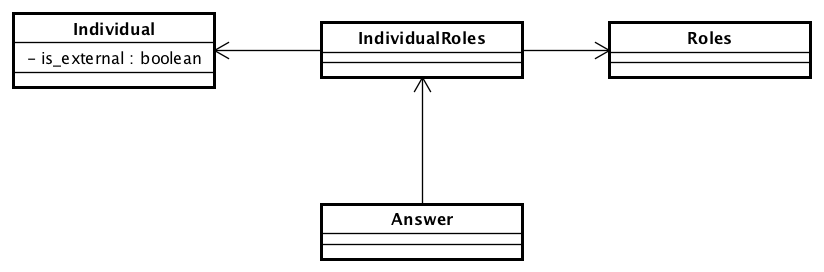
\includegraphics[width=12cm]{Pics/UMLClassiFigureDiSistema.png}
				\caption{
					Diagramma delle classi per la gestione delle figure di sistema ed i relativi questionari.}
				\label{fig:DiagrammaDelleClassiIndividualRoles}
			\end{center}
		\end{figure}
	Obiettivo primario del refactor è stato centralizzare tutte le informazioni relative alle figure di sistema ed i loro questionari in un unica sezione. 
	La schermata presente nella  \autoref{fig:ScreenPrincipaleFigureDiSistema} vuole rappresentare il risultato del lavoro svolto per le figure riguardanti l'azienda. \\
		\begin{figure}[H]
			\begin{center}
				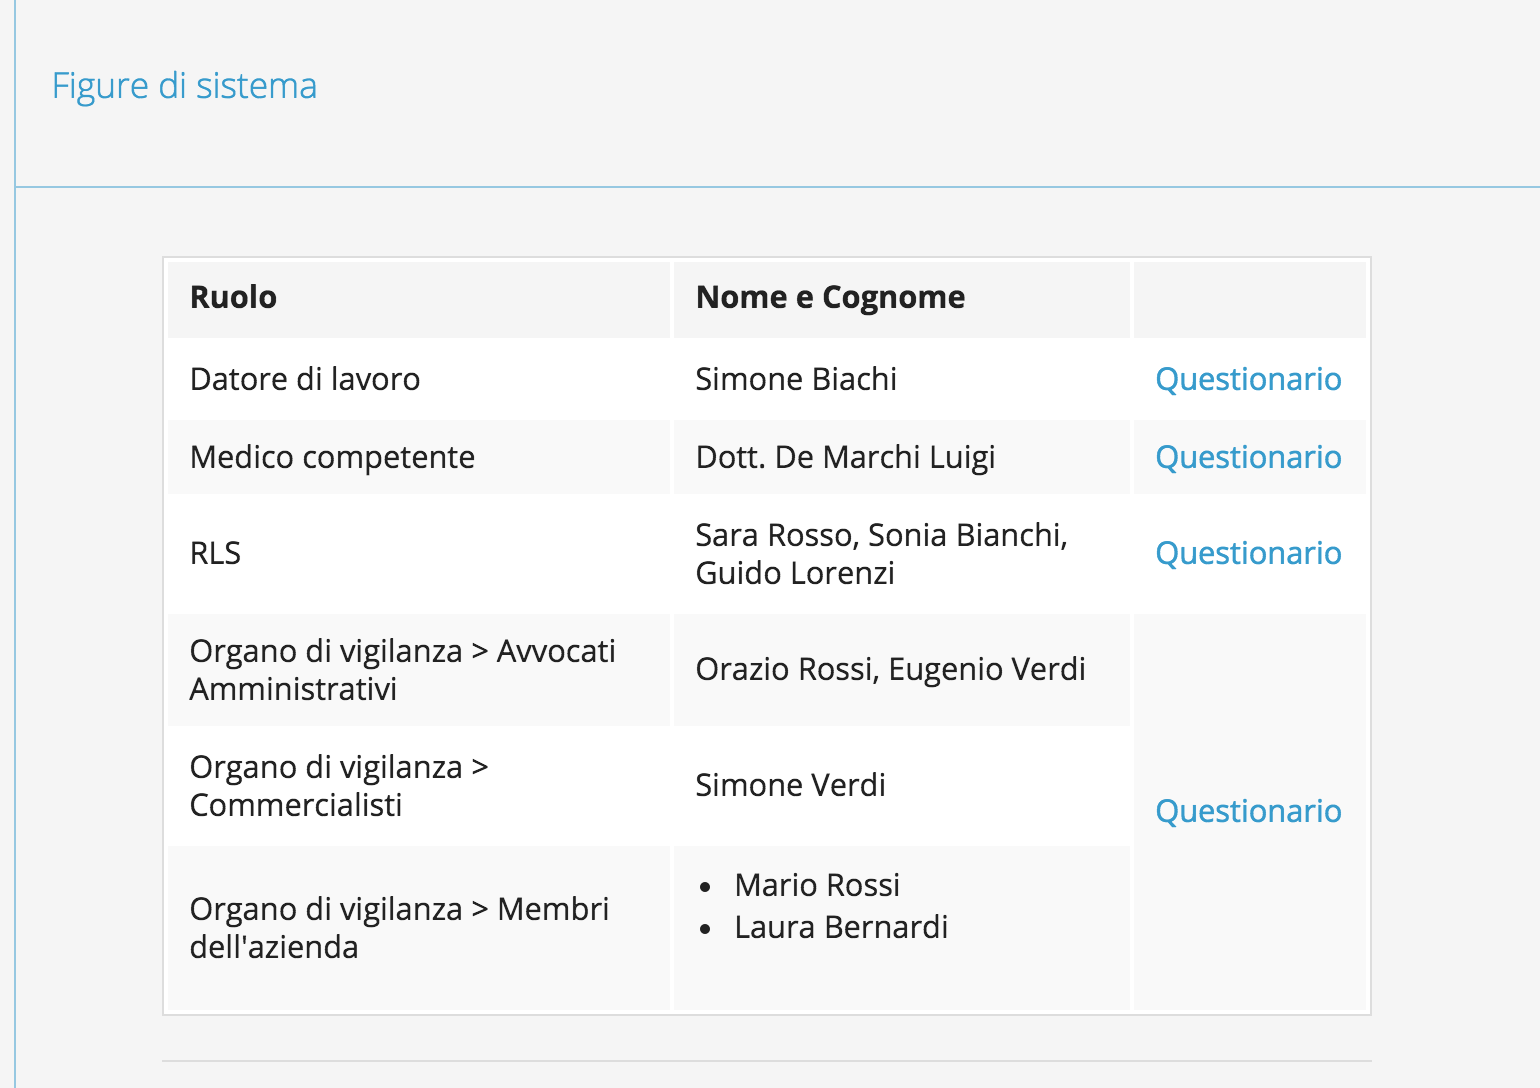
\includegraphics[width=12cm]{Pics/ScreenFigureDiSistemaProspetto.png}
				\caption{
					Schermata iniziale della sezione \textit{Figure di sistema}.}
				\label{fig:ScreenPrincipaleFigureDiSistema}
			\end{center}
		\end{figure}
	È stato implementato inoltre un pannello dedicato alla gestione delle figure impiegate in specifiche sedi o cantieri. In questo modo è sempre possibile allocare gli individui nei luoghi d'interesse senza vincoli di molteplicità.\\
	\begin{figure}[H]
		\begin{center}
			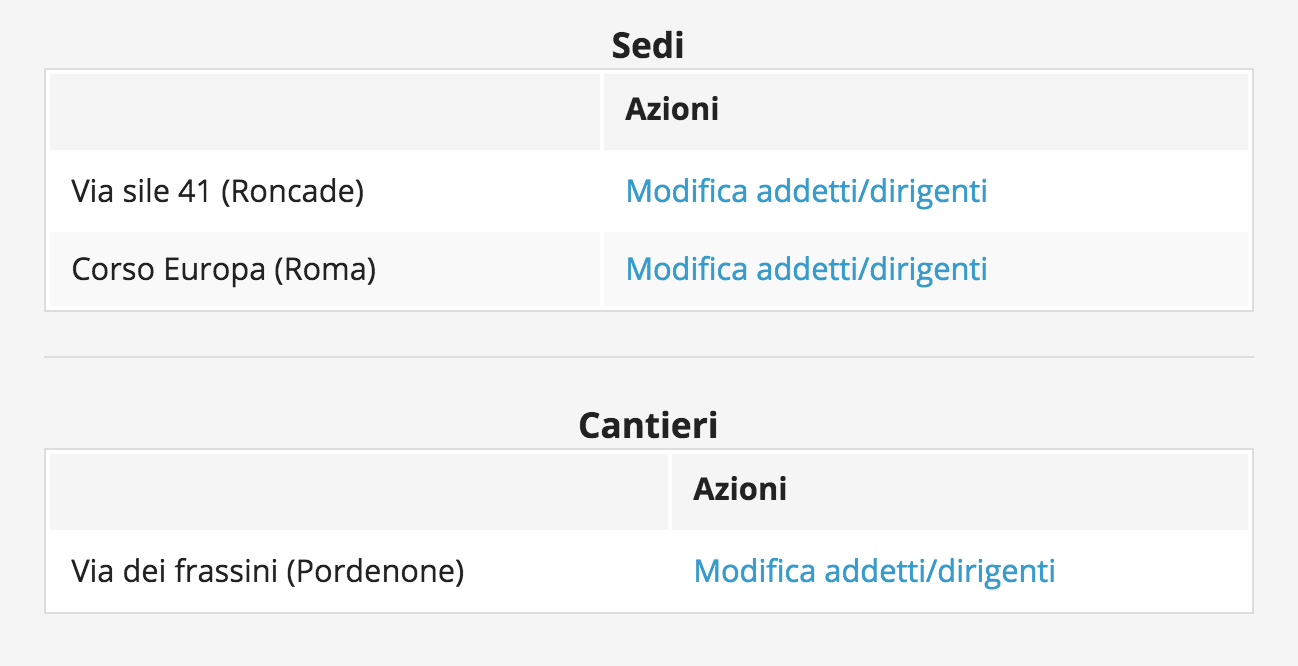
\includegraphics[width=12cm]{Pics/ScreenfigureDiCantiere.png}
			\caption{
				Schermata iniziale della sezione \textit{Pannnello di gestione delle figure impegnate in sedi e cantieri.}.}
			\label{fig:ScreenPrincipaleFigureSediCantieri}
		\end{center}
	\end{figure}

	Per facilitare l'inserimento delle informazioni relative alla selezione dei dipendenti, è stata utilizzata la libreria \textit{Selectize.js} per rendere i form più gradevoli dal punto di vista grafico e per permettere l'autocompletamento (vedi \autoref{fig:ScreenOrganodiVigilanza} ). \\ 
	Una criticità si è presentata nell'inserimento dinamico delle figure che possono essere presenti con molteplicità maggiore di uno. In particolare gli RSPP e gli ASPP presentano l'ulteriore complicazione rappresentata dal fatto che possono essere sia membri interni all'azienda, sia esterni. \\
	In entrambi i casi, la situazione è stata gestita mediante chiamate \gls{Ajax}, evitando quindi di dover ricaricare la pagina ad ogni inserimento e generando un record della classe \textit{Individual}  identificato da un particolare flag (\texttt{is\_external}) nel caso si tratti di una figura esterna all'azienda.\\
	\newpage
	\begin{figure}[H]
		\begin{center}
			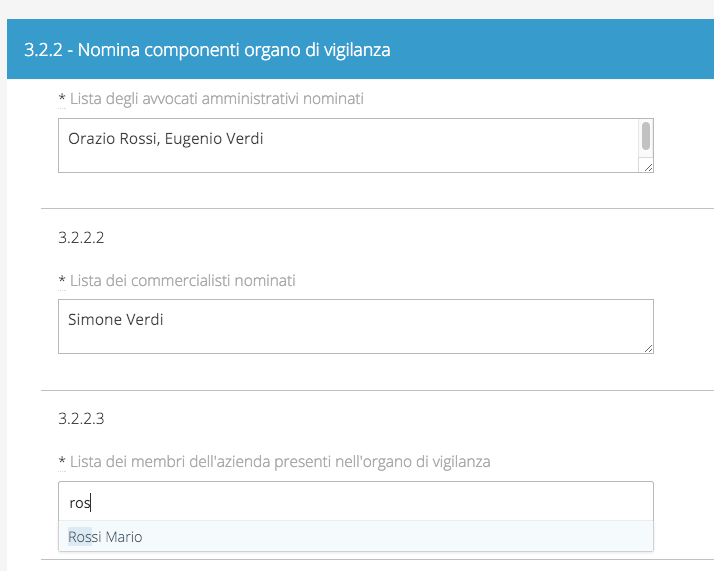
\includegraphics[width=12cm]{Pics/screen_organo_di_vigianza_con_autocompletamento.png}
			\caption{
				Schermata relativa all'inserimento di alcune informazioni in merito all'organo di vigilanza}
			\label{fig:ScreenOrganodiVigilanza}
		\end{center}
	\end{figure}
	
	Ad ogni figura di sistema è stato associato un questionario nel quale sono specificate le informazioni in merito alla carica, tra tutte la data di accettazione e scadenza dell''incarico.
	\begin{figure}[H]
		\begin{center}
			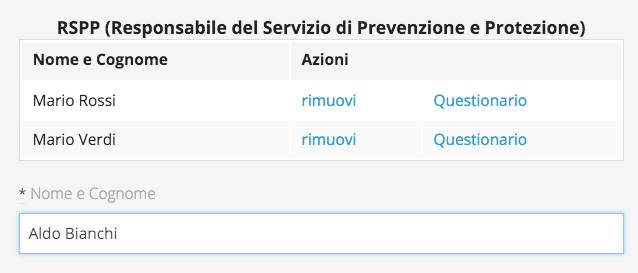
\includegraphics[width=12cm]{Pics/RemoteTrueRSPP.png}
			\caption{
				Schermata relativa all'inserimento di un RSPP.}
			\label{fig:ScreenRSPP}
		\end{center}
	\end{figure}	
	  L'associazione ad un questionario avviene generando tutte le risposte ad esso relative.\\
	  Per ogni risposta saranno preimpostati i seguenti valori:
	  \begin{itemize}
		  \item \texttt{response:} \texttt{nil};
		  \item \texttt{answerable\_type:} \texttt{"IndividualRoles"};
		  \item \texttt{answerable\_id:} codice identificativo dell'istanza specifica di \texttt{"IndividualRoles"}.
	  \end{itemize}

	Facendo Riferimento alla \autoref{fig:ScreenRSPP} e  supponendo che \textit{Aldo Bianchi} non sia attualmente presente nel database, alla pressione del tasto invio verrà generato un nuovo \textit{Individual} relativo ad \textit{Aldo Bianchi}. Successivamente verrà generato un questionario con le domande relative agli RSPP in relazione ad \textit{Aldo Bianchi}.
	
\newpage
\subsubsection{Refactor della componente: \textit{Dispositivi di protezione individuale}}
\newpage
\subsubsection{Refactor della componente: \textit{Mansioni e formazioni correlate}}
\newpage
\subsubsection{Refactor della componente: \textit{Questionari}}

\newpage
\subsection{Nuove componenti}
\subsubsection{\textit{Segnalazioni}}
%parlare del fatto che sono ufficiali e che sollevano il segnalante dalla responsabilità se era sua
	\paragraph{Requisiti}
	\paragraph{Progettazione}
	\paragraph{Criticità incontrate}
\newpage
\subsubsection{\textit{Procedure}}
	\paragraph{Requisiti}
	\paragraph{Progettazione}
	\paragraph{Criticità incontrate}
		%più controller e viste associate allo stessa categoria, uno ha il modello l'altro il questionario
\newpage
\subsubsection{\textit{Dispositivi di protezione collettivi}}
	\paragraph{Requisiti}
	\paragraph{Progettazione}
	\paragraph{Criticità incontrate}
		%remote true
		

\newpage
\subsection{Regole Drools}

\newpage
\section{Verifica e validazione}
\newpage
\section{Considerazioni finali}